\section{Evaluation}\label{sec:eval}
We evaluated our MPI and hybrid implementations of \rs{}, \block{}, and \fw{}
with strong scaling studies across a range of problem sizes. For \rs{} and
\block{}, we used a baseline of \rsomp{}, which has access to 24 threads. For
\fw{}, we used a baseline of \fwomp{}, which has access to 24 threads. For
\rs{} and \block{}, we also performed a weak scaling study with a constant
amount of work per thread corresponding to a graph of size $N=500$.

\subsection{RS}
\subsubsection{MPI}
In \figref{strong-rs-mpi}, we can see that increasing the number of MPI ranks,
which in turn decreases the number of OMP threads per rank, does increase
speedup, but for any problem size larger than 960 does not get above 1. Further
there is a drop when ranks goes beyond 12. This is because of increased MPI
overhead across 2.

In weak scaling (\figref{weak-rs-mpi}) we that performance per thread drops
as speedup falls. This is likely because of the increased overhead of
synchronizing with 1 more thread as we add 1 more thread.

\subsubsection{Hybrid}
In \figref{strong-rs-hybrid} we can see that increasing the number of MPI
ranks (which in turn decreases the number of OMP threads per rank) has mixed
speedup for most n. When the number of MPI ranks is less than 10 we sometimes
have speedup larger than 1, but as we go beyond 10 and 12 speedup drops off.
This is because of increased MPI overhead across 2 chips and the hybrid codes
inability to take advantage of all possible threads when there are more than 12
MPI ranks.

The hybrid implementation drops speedup more rapidly than the MPI implementation
for weak scaling (\figref{weak-rs-hybrid}). This is probably because
inability to take advantage of the full 24 hardware threads when the number of
ranks does not divide 24 perfectly.

\subsection{Block}
\subsubsection{MPI}
Our block implementation with MPI has much higher speedups than our repeated
squares with MPI. It crosses 5x speedup for almost all problem sizes at some
point (figure~\ref{strong-block-mpi}). In particular we see that smaller
problems (960 being a notable outlier) with larger speedup. Speedup once again
increases until 12 and then drops (due to multiple chips) and then increases
once again.

\subsubsection{Hybrid}
Our block implementation with hybrid has much higher speedups than our repeated
squares with hybrid, however the speedups are smaller than for MPI
(figure~\ref{strong-block-hybrid}). Speedup varies between sizes, particular
with fewer than 12 ranks due to not always taking advantage of all 24 hardware
threads. Once again, problem size 960 has much more speedup than other sizes.

\subsection{FW}
\subsubsection{MPI}
The performance of FW with MPI is typically poor, this is because of the
increased number of synchronizations ($O(N)$) as compared to to $O(log(N))$. We
see this in figure~\ref{strong-fw-mpi}, speedup slowly increases for all sizes,
but in all cases except for the smallest size (480), never surpasses one; in
fact, all but 480 and 960 never cross 0.5 speedup.

\subsubsection{Hybrid}
The performance of FW with hybrid actually tends to decrease as ranks increase,
this is because of the increased number of synchronizations once again along
with inability to use all 24 hardware threads. We see this in
figure~\ref{strong-fw-hybrid}.

% label
% strong-filename
% strong-caption
% weak-filename
% weak-caption
\newcommand{\sidebyside}[5]{
  \makebox[\textwidth][c]{
    \begin{subfigure}[c]{0.5\textwidth}
      \centering
      \includegraphics[width=\textwidth]{#2}
      \caption{#3}
      \label{fig:strong-#1}
    \end{subfigure}
    \quad
    \begin{subfigure}[c]{0.5\textwidth}
      \centering
      \includegraphics[width=\textwidth]{#4}
      \caption{#5}
      \label{fig:weak-#1}
    \end{subfigure}
  }
}

\begin{figure}
  \centering
  \sidebyside{rs-mpi}
    {plots/strong_rs-mpi_baseline-rs-omp--1.pdf}
    {\rsmpi{} strong scaling (\rsomp{} baseline)}
    {plots/weak_rs-mpi.pdf}
    {\rsmpi{} weak scaling}
  \sidebyside{rs-hybrid}
    {plots/strong_rs-hybrid_baseline-rs-omp--1.pdf}
    {\rshybrid{} strong scaling (\rsomp{} baseline)}
    {plots/weak_rs-hybrid.pdf}
    {\rshybrid{} weak scaling}
  \sidebyside{block-mpi}
    {plots/strong_block-mpi_baseline-rs-omp--1.pdf}
    {\blockmpi{} strong scaling (\rsomp{} baseline)}
    {plots/weak_block-mpi.pdf}
    {\blockmpi{} weak scaling}
  \caption{\rsmpi{}, \rshybrid{}, and \blockmpi{}}
\end{figure}

\begin{figure}
  \centering
  \sidebyside{block-hybrid}
    {plots/strong_block-hybrid_baseline-rs-omp--1.pdf}
    {\blockhybrid{} strong scaling (\rsomp{} baseline)}
    {plots/weak_block-hybrid.pdf}
    {\blockhybrid{} weak scaling}
  \sidebyside{fw}
    {plots/strong_fw-mpi_baseline-fw-omp--1.pdf}
    {\fwmpi{} strong scaling (\fwomp{} baseline)}
    {plots/strong_fw-hybrid_baseline-fw-omp--1.pdf}
    {\fwhybrid{} strong scaling (\fwomp{} baseline)}
\end{figure}

\begin{figure}
  \centering
  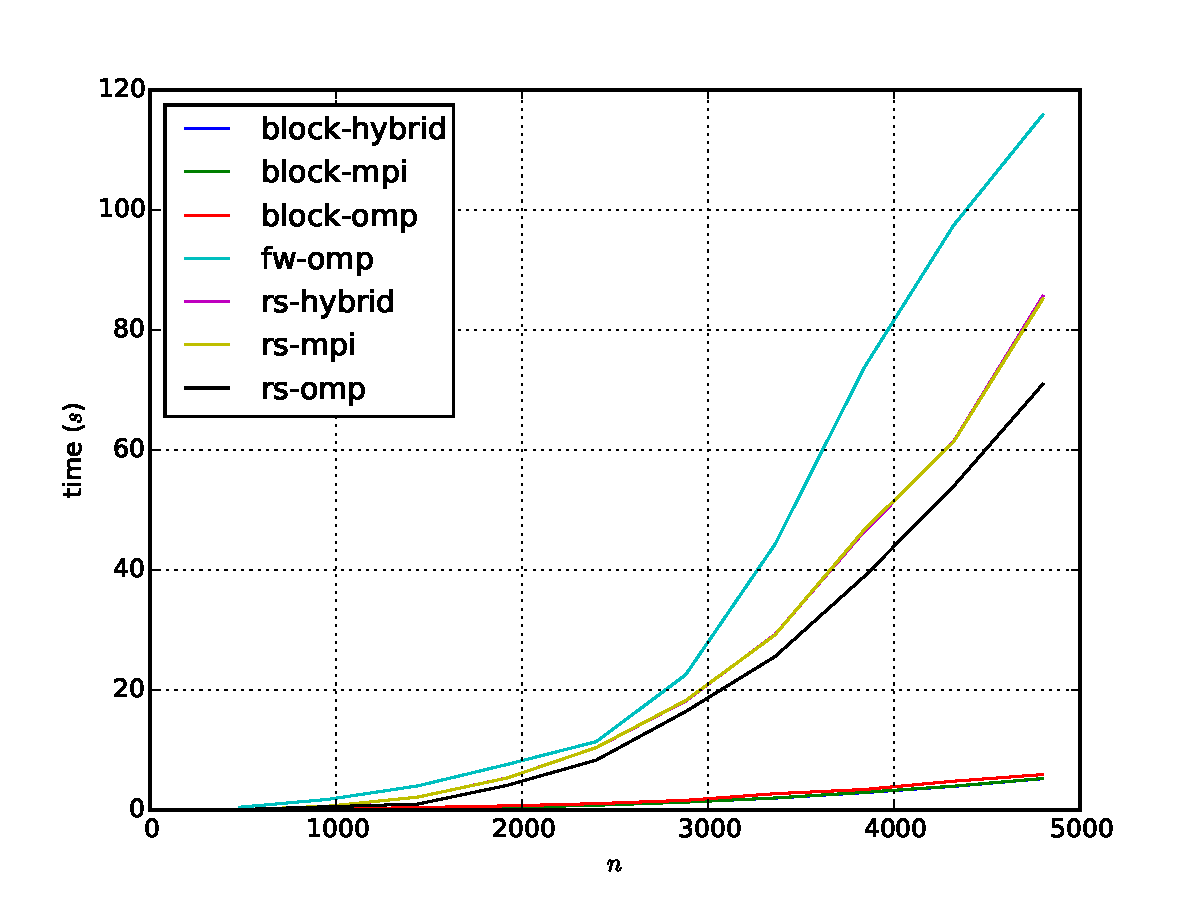
\includegraphics[width=\textwidth]{plots/all.pdf}
  \caption{%
    Performance comparison of all algorithms excluding \fwmpi{} and \fwhybrid{}.
  }
  \label{fig:perf}
\end{figure}
